\documentclass[a4paper,12pt]{article}

\usepackage{graphicx}	% Pour importer des images
\usepackage[left=2.5cm,right=2.5cm,top=2cm,bottom=3.5cm]{geometry} %Configuration de la page
\usepackage{amsmath}
\usepackage{amsthm}
\usepackage{hyperref}
\usepackage{float}
\usepackage{booktabs}
\usepackage[T1]{fontenc}
\usepackage[table]{xcolor}
\newtheorem*{remark}{Remark}


\begin{document}

\title{Note on Hypotension Prediction}

\author{Bob Aubouin--Pairault}
\maketitle


\section{Goal of the document}

The goal of this document is to summarize all the work done on the hypotension prediction.


\section{Abstract sent to the conference}

Intraoperative hypotension (IOH) is common during surgical procedures. It may be caused by anesthesia drugs, underlying  comorbidities of the patient such as heart failure, or by the surgical procedure. There are strong associations between IOH and postoperative organ complications, thus the ability to predict IOH to support the clinician is an attractive prospect. In this presentation, the prediction of hypotension during general anesthesia using physiological signal is investigated. \medskip

Recently, some research has been focused on trying to predict hypotension events occurring during surgeries using machine learning techniques \cite{hatibMachinelearningAlgorithmPredict2018}. However, this methodology has been subject to some questioning \cite{enevoldsenPerformanceHypotensionPrediction2022}, \cite{smithConHypotensionPrediction2023}. Especially, the database seems to be biased, and the evaluations are not compared to a relevant baseline. A new methodology addressing the arisen questions is proposed here. Exploratory investigations are illustrated using the open source VitalDB database \cite{leeVitalDBHighfidelityMultiparameter2022} and standard machine learning algorithms. In addition, the explainability of the prediction is studied to provide more information to the anesthesiologist.


\section{Feature selection}


\begin{table}
\small
\begin{center}
\center
\rowcolors{2}{white}{gray!20}
\begin{tabular}{p{0.17\textwidth}|p{0.4\textwidth}|c|c}
\textbf{Feature} & \textbf{Description} & \textbf{VitalDB Name} & \textbf{Code name} \\
\midrule
Mean Arterial Pressure & Average blood pressure during a cardiac cycle & Solar8000/ART\_MBP & mbp\\
Systolic Blood Pressure & Maximum blood pressure during a cardiac cycle & Solar8000/ART\_SBP & sbp \\
Diastolic Blood Pressure & Minimum blood pressure during a cardiac cycle & Solar8000/ART\_DBP & dbp \\
Heart Rate & Number of heart beats per minute & Solar8000/HR & hr\\
Respiration Rate & Number of breaths per minute & Solar8000/RR & rr\\
Oxygen Saturation & Percentage of hemoglobin saturated with oxygen & Solar8000/PLETH\_SPO2 & spo2 \\
End Tidal CO2 & Concentration of carbon dioxide at the end of an exhaled breath & Solar8000/ETCO2 & etco2 \\
Propofol target & Target of propofol concentration in the blood & Orchestra/PPF20\_CT & pp\_ct\\
 MAC & minimum alveolar concentration (MAC), for volatile anesthetics &  Primus/MAC & mac\\
 BIS & Bispectral index (depth of hypnosis) & BIS/BIS & bis
\end{tabular}
\caption{List of the dynamic features that can be linked to the prediction of hypotension.}
\end{center}
\end{table}

\begin{table}
\begin{center}
\rowcolors{2}{white}{gray!20}
\begin{tabular}{c|p{0.4\textwidth}|c}
\textbf{Feature} & \textbf{Description} & \textbf{VitalDB Name} \\
\midrule
Age & Age & age \\
BMI & Body mass index & bmi \\
ASA & Physical statut classification & asa \\
Creatinine & Preoperative creatinine concentration in the blood & preop\_cr \\
Hypertension & Preoperative hypertension of the patient & preop\_htn \\
operation name & operation name (if we can proceed text) & opname
\end{tabular}
\caption{List of the static features that can be linked to the prediction of hypotension.}
\end{center}
\end{table}

\section{Patient selection}
Patients are selected using the following criteria:

\begin{itemize}
    \item The patient is under general anesthesia
    \item The patient is not in emergency
    \item Arterial blood pressure is invasively measured
    \item The patient is major (age > 18yr)
    \item The operation is not a transplantation (no "transplant" in operation name
    \item The anesthesia duration is at least one hour.
    \item More than 70\% of the previously listed signals are available (no Nan) 
    \item All the static information about the patient are available
\end{itemize}

\section{Labelling the data}
As there is no clear adopted definition of hypotension event automatic labelling of the data could be an arduous task. In the literature, it exists two different quantitative ways to define hypotension: using a relative threshold from baseline of mean or systolic blood pressure or using an absolute threshold on those value. Because the true blood pressure baseline might be hard to obtain, the first method is often inapplicable in practice. The second method, easier to implement is actually used for most of the research papers on this topic. However, this labelling method lacks of patient specificity, in fact, the baseline MAP of some patient patient might be close to the threshold such that labelled situation could correspond to normal situation. \medskip

For our approach, a new method for labelling the hypotension events is proposed. Our guess is that the anesthesiologists in the surgery room are the more appropriate to diagnostic IOH. Thus, the idea is to take advantage of our future point of view to asses the potential of a low blood pressure to correspond to an IOH thanks to the anesthesiologist reaction in the minutes following the event. \medskip

To treat an IOH event different possibilities can used depending on the cause:
\begin{itemize}
    \item If the IOH is due to a too deep hypnosis, the hypnotic drug dosage must be adjusted.
    \item If the IOH is due to a too important fluid loss, the missing fluid must be replaced with blood or cristalloid.
    \item If the cause is the vasodilatation of the vessels, vasopressor drugs must be injected.
\end{itemize}

The first possibility can be verified easily using data from hypnotic drug dosage (i.e. propofol, desflurane or sevoflurane). The second also correspond to changes in drug injection profiles. However of those drug are mostly injected by bolus and only the total amount of drug injected during the anesthesia is recorded in vitalDB. The same problem apply to fluid replacement where only the total amount of fluid lost and injected is available in vitalDB.




\section{Data pre-processing}

First, to remove time where arterial blood pressure is not monitored, all the sample where MAP<40mmHg are removed. In addition, to remove peak values, sample where MAP >150 are also removed.

For physiological signal, missing value are replaced by last valid measured value. For drug rates value and MAC missing values are replace by last valid value or 0 if no measures are available.



\section{Evaluation}

To fairly evaluate the potential of our method against baseline and evaluate uncertainty on our results a Leave One Out Cross-Validation (LOOCV) is used \cite{meghnoudjSparseOptimalControlbased2024}. This method consist on partitioning the set of patient in $k$ distinct subset. Then to loops are nested, in the outer one a subset is leaved out before any training on the data and is used as a test set to asses the performance of the method. In the inner one, a subset is leaved out to be used as a validation set for the hyperparameters tuning. This method is illustrated on Fig.~\ref{fig:loocv}.

\begin{figure}
    \centering
    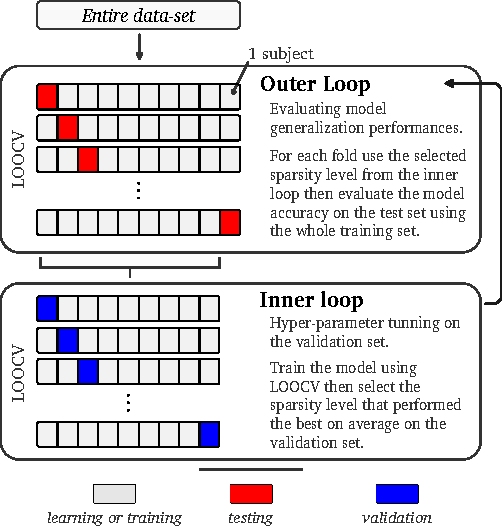
\includegraphics[width=0.7\textwidth]{figures/chap_1_NLOO.pdf}
    \caption{Illustration of Leave one out cross validation (from \cite{meghnoudjSparseOptimalControlbased2024})}
    \label{fig:loocv}
\end{figure}

In this work the metric used is the Aera Under the Receiver operating characteristic curve (AUC). This curve evaluate the ability of a binary classifier at different threshold value and is usually used in medical field. It is the plot of the True Positive error against the False positive error (or sensitivity against 1 - specificity).

\section{Baseline}


For IOH prediction, the baseline must be the ability of the mean arterial pressure to predict the events. In fact it is this value that is currently on the clinicals monitors and used by the 


\bibliographystyle{ieeetr}
\bibliography{bibli}


\end{document}
